\section{Results and discussion}\label{sec:rnd}

\begin{figure}%[h]
\centering
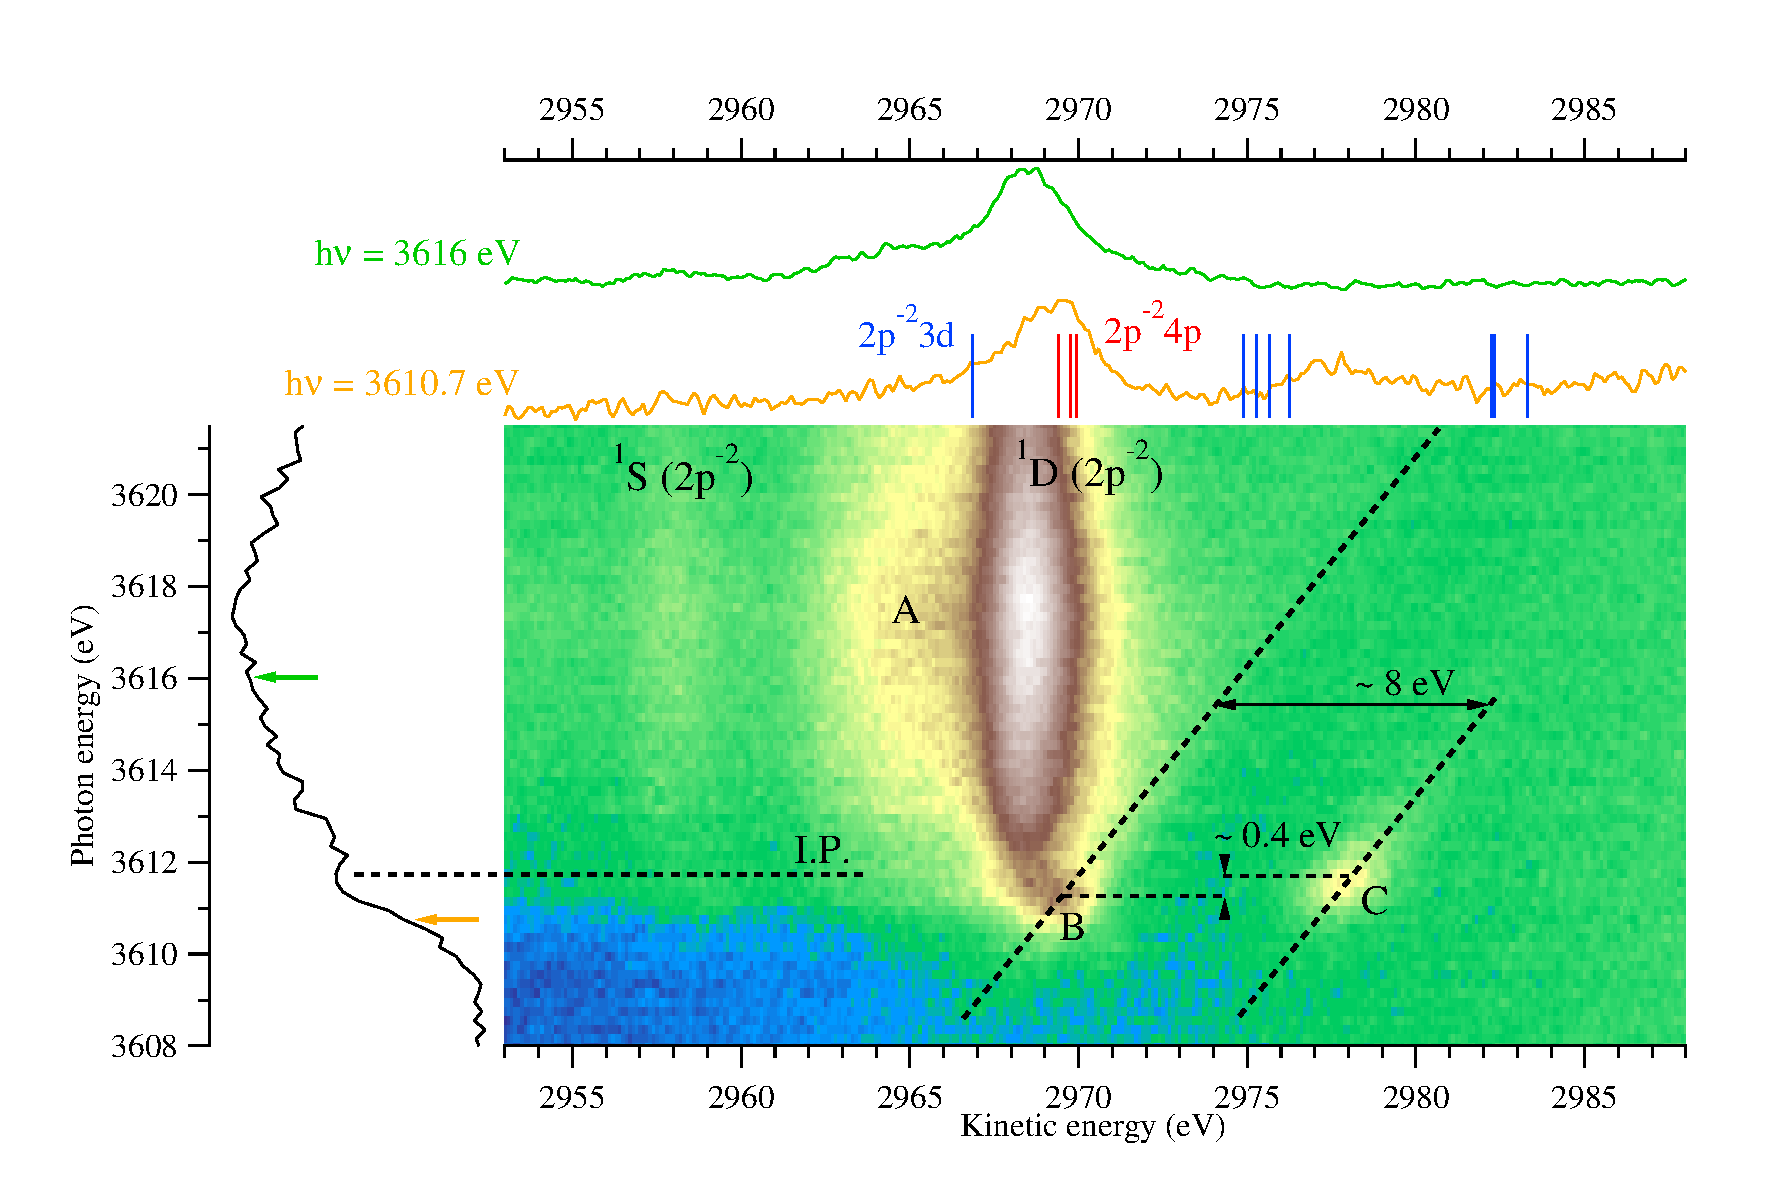
\includegraphics[scale=0.55]{figures/k_2dmap.pdf}
\caption{2D map showing the kinetic energy of the electrons emitted in KL$_{2,3}$L$_{2,3}$ Auger decay vs the photon energy in the vicinity of the K-edge of aqueous K$^{+}$. The black curve on the left represents the experimental partial electron yield spectrum of K$^{+}$ obtained after integrating over the kinetic energies of the Auger electrons in the energy range presented on the figure. The upper panel shows two spectra at photon energies 3610.7\,eV, and 3616\,eV below and above the ionization potential at 3611.9\,eV, respectively. The bars in the pre-edge cut correspond to the final 2p$^{-2}$ 3d (blue) and 2p$^{-2}$4p (red) doublet resonant Auger states of K$^{+}$(H$_2$O)$_6$ computed at the CIS level (see Sec.\ \ref{sec:methods} for details). The features A, B and C are discussed in the text.}
\label{fg:2dmap_k}
\end{figure}


\begin{figure}%[h]
\centering
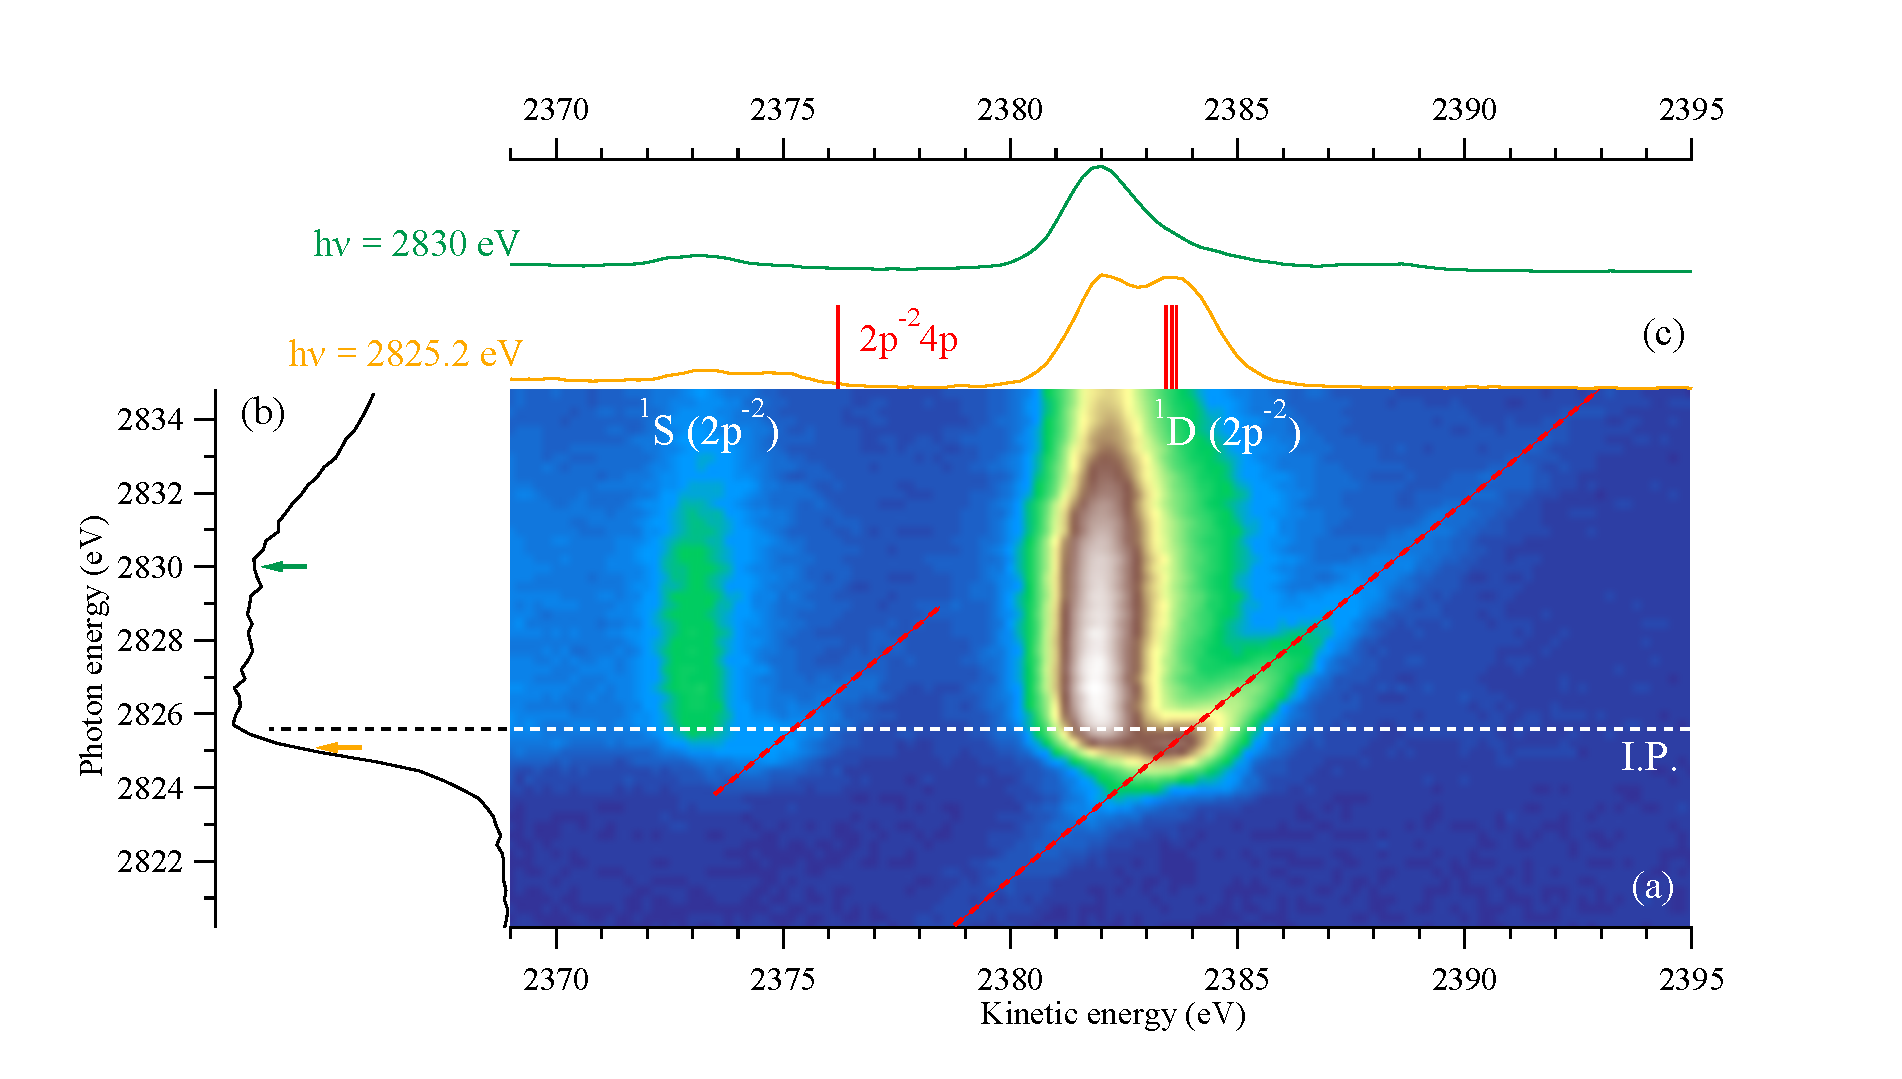
\includegraphics[scale=0.55]{figures/cl_2dmap.pdf}
\caption{2D map showing the kinetic energy of the electrons emitted in KL$_{2,3}$L$_{2,3}$ Auger decay vs the photon energy in the vicinity of the K-edge of aqueous Cl$^{-}$. The black curve on the left represents the experimental partial electron yield spectrum of Cl$^{-}$ obtained after integrating over the kinetic energies of the Auger electrons in the energy range presented on the figure. The upper panel shows two spectra at photon energies 2825.2\,eV, and 2830.0\,eV below and above the ionization potential at 2825.4\,eV, respectively. The bars in the pre-edge cut correspond to the final 2p$^{-2}$ 3d (blue) and 2p$^{-2}$4p (red) doublet resonant Auger states of Cl$^{-}$(H$_2$O)$_6$ computed at the CIS level (see Sec.\ \ref{sec:methods} for details).}
\label{fg:2dmap_cl}
\end{figure}


\subsection{Normal Auger decay}\label{ssec:na}

The KL$_{2,3}$L$_{2,3}$ normal Auger decay following K-shell ionization of aqueous \ki~and \cli~can be written as follows
%
\begin{align*}
\gamma + \text{K}^{+}_{\text{aq}} \rightarrow \text{K}^{2+}_{\text{aq}} (1s^{-1}) \rightarrow \text{K}^{3+}_{\text{aq}} (2p^{-2}) + e^{-}_{\text{Auger}}\\
\gamma + \text{Cl}^{-}_{\text{aq}} \rightarrow \text{Cl}^{0}_{\text{aq}} (1s^{-1}) \rightarrow \text{Cl}^{+}_{\text{aq}}(2p^{-2}) + e^{-}_{\text{Auger}}
\end{align*}
%
It results in the population of 2p$^{-2}$($^3$P, $^1$D, $^1$S) final states. 
%The $^3$P final states are not observed in the experiment since they are forbidden from parity conservation rules.
The $^3$P final states are expected to have a very low intensity since at the first order they are forbidden from parity conservation rules. In addition, in the photon energy range of interest, the tail of the $^1$D state described in the next paragraph, and the $^1$D 2p$^{-2}$V' dispersive state (see next section) {\color{red}overlap with the $^3$P state in the kinetic energy region where it is expected to occur, thus making it impossible to properly determine its position.} In the case of K$^{+}_{\text{aq}}$ the maxima of the $^1$S and $^1$D KL$_{2,3}$L$_{2,3}$ Auger lines are located at 2958\,eV and 2968.4\,eV, respectively (see Fig.\ \ref{fg:2dmap_k}). For Cl$^{-}_{\text{aq}}$, the lines corresponding to the Cl$^{+}$ (2p$^{-2}$) $^1$S and $^1$D states are located at 2373.2\,eV and 2382.1\,eV kinetic energy (see Fig.\ \ref{fg:2dmap_cl}).


The KL$_{2,3}$L$_{2,3}$ Auger lines do not disperse with photon energy except close to threshold due to the interaction between the photoelectron and Auger electron, i.e.\ the so-called post-collision interaction (PCI). As a result of this interaction, first, the peaks in the Auger spectrum become asymmetric with a shoulder at high kinetic energies, and second, they are shifted to higher kinetic energies close to threshold \citep{russek86:911,guillemin15:012503}. Consequently, one can attribute the high kinetic energy shoulder of the $^1$D and $^1$S peaks on Figs.\ \ref{fg:2dmap_k} and \ref{fg:2dmap_cl} as resulting from PCI effect. {\color{red}The asymmetric tail of the peaks resulting from PCI can be clearly seen on the cuts taken at photon energies 3616\,eV in the case of \ki, and 2830\,eV in the case of \cli.}


%In order to quantify this effect we recorded the KLL Auger spectrum of both Cl$^{-}_{\text{aq}}$ and K$^{+}_{\text{aq}}$ at higher photon energies, $h\nu = 5$\,keV (see Ref.\ \citep{ceolin17:263003} for details). In this case, the maxima of the $^1$D and $^1$S states were found at 2381.1\,eV and 2372.3\,eV for Cl$^{-}_{\text{aq}}$, and 2967.4\,eV and 2957\,eV kinetic energy for K$^{+}_{\text{aq}}$, respectively. The lines observed at photon energies far from threshold and close to it appear to be shifted by $\sim$1\,eV. The magnitude of the shift is the same for both ions suggesting that it does not depend on the initial charge of the ion, and it is almost constant in the photon energy range presented here.
% Jan 24 Tsveta
Further, we compare the positions of the normal KLL Auger lines of both Cl$^{-}_{\text{aq}}$ and K$^{+}_{\text{aq}}$ close to threshold with those recorded far from threshold, at photon energies $h\nu = 5$\,keV (see Ref.\ \citep{ceolin17:263003} for details). In this case, the maxima of the $^1$D and $^1$S states were found at lower values at 2381.1\,eV and 2372.3\,eV for Cl$^{-}_{\text{aq}}$, and 2967.4\,eV and 2957\,eV kinetic energy for K$^{+}_{\text{aq}}$, respectively. The lines observed at photon energies far from threshold and close to it appear thus to be shifted by $\sim$1\,eV. The magnitude of the shift is the same for both ions suggesting that it does not depend on the initial charge of the ion, and it is almost constant in the photon energy range presented here.
A possible explanation of the shift observed in our experiment is given in Ref.\ \cite{tchaplyguine07:124314}, which focuses on the Auger decay of large Kr clusters on and just above the 3d$_{5/2}$ ionization threshold. The observed 4d$^{4}$($^1$D) Auger peak was found to be shifted by 0.7\,eV to higher kinetic energies compared to the position of the peak far above threshold. Moreover, the shift did not vary with the photon energy close to threshold. Consequently, it was proposed that this feature originates from a process of internal ionization, i.e.\ excitation of the photoelectron into the conduction band. Further investigations are, however, planned in the case of liquid samples.
%\denis{A possible explanation was given in the reference M. Tchaplyguine et al., The Journal of Chemical Physics 127, 124314 (2007) focusing on the Auger decay of large Kr clusters following ionization of the 3d$_{5/2}$ orbital. Considering that the observed PCI shift was not varying with the photon energy close to threshold, a process of excitation of the photoelectron into the conduction band was thus proposed. Further investigation are however planned in the case of liquid samples.}
% The observed PCI shift of 1\,eV is larger than in the case of the isoelectronic Ar, where its value is $\sim$0.5\,eV at a photon energy of 10 \,eV above threshold \citep{guillemin15:012503}. The shift in the energies of the photo- and Auger electrons is proportional to the change in the ionic field during the Auger process. In a solution, both the single and double ionization potentials change due to the polarization of the water molecules and the stabilization of the ionic species through ion-dipole interaction with the polarized solvent. For example, in \ki, the ionization potential of the bare ion was experimentally determined to be 3619.4\,eV \citep{hertlein06:062715}, whereas in an aqueous solution, its value drops by about 7.5\,eV. The magnitude of this effect increases with the ionic charge, consequently, there will be an even greater difference for the double ionization potential. Thus, one can expect a larger change in the ionic field in an aqueous solution compared to that in a Van der Waals cluster, which can, therefore, account for the large PCI shift of the Auger lines in a solution.

Finally, the normal Auger $^1$D main line of K$^{+}$ differs from that of Cl$^{-}$ by the presence of a large shoulder (A on Fig.\ \ref{fg:2dmap_k}) on the low kinetic energy side at about 2965\,eV kinetic energy. This shoulder is attributed to electron transfer from the water solvent molecules \citep{ceolin17:263003} to the 3d orbital of K$^{+}$. In the case of \cli, there is no experimental evidence of such intense electron transfer processes.


\subsection{Resonant Auger decay} \label{ssec:ra}

%\kolya{XAS of Cl- and K+ from previous works?}

The KL$_{2,3}$L$_{2,3}$ Auger decay following resonant K-shell excitation of solvated \ki~and \cli~can be written as follows
%
\begin{align*}
\gamma + \text{K}^{+}_{\text{aq}} \rightarrow \text{K}^{+*}_{\text{aq}} (1s^{-1}V) \rightarrow \text{K}^{2+}_{\text{aq}} (2p^{-2}V') + e^{-}_{\text{Auger}}\\
\gamma + \text{Cl}^{-}_{\text{aq}} \rightarrow \text{Cl}^{-*}_{\text{aq}} (1s^{-1}V) \rightarrow \text{Cl}^{0}_{\text{aq}}(2p^{-2}V') + e^{-}_{\text{Auger}}
\end{align*}
%
where $V$ and $V'$ denote the unoccupied orbitals in the excited and singly ionized excited states, i.\ e.\ in the presence of the 1s$^{-1}$ and 2p$^{-2}$ core holes. The character of these states is discussed below.

{\color{red}How are the IPs determined? 2D maps reveal the core excited states.}
The pre-edge regions of the x-ray absorption spectra of \ki~and \cli~shown to the left on Figs.\ \ref{fg:2dmap_k} and \ref{fg:2dmap_cl} do not exhibit any high intensity features due to the lifetime broadening and energetic proximity of the core excited states to the ionization threshold. Consequently, solely from these absorption spectra, one cannot conclude whether there are core excited states in the pre-edge structure, which can undergo resonant Auger decay. However, one can determine their excitation energies from the maxima of the resonant Auger features. Thus, for \cli, the lowest core excited state is located at 2825.2\,eV, which agrees very well with the position of the Cl$^{-}$ 1s$\,\rightarrow\,$4p excitation determined from Cl K-edge XAS experiments in MgCl$_2$.6H$_2$O and of SrCl$_2$/SrCl$_2$.6H$_2$O \citep{sugiura82:681} and MCl$_{4}^{-}$ compounds \citep{shadle95:2259}. In the case of \ki, there are two dispersive features with maxima at photon energies of 3611.2\,eV (B) and 3611.6\,eV (C), respectively (Fig.\ \ref{fg:2dmap_k}). The positions of these two core excited states are close to the energy of the 1s$\,\rightarrow\,$4p excitation in bare \ki, 3610.7\,eV \citep{hertlein06:062715}.


%Unlike the normal Auger decay, which proceeds in a fairly similar way in the two ions, 
The resonant Auger features produced in the decay of these core excited states appear to be quite different for \cli~and \ki. In the spectrum of \cli~shown in Fig.\ \ref{fg:2dmap_cl} there are two dispersive features on the high kinetic energy side of the main $^1$S and $^1$D lines, i.e.\ at 2825.2\,eV photon energy and 2374.6 and 2383.4\,eV kinetic energy. In the case of \ki, the $^1$S dispersive line cannot be clearly identified due to the presence of strong background. The dispersive feature close to the $^1$D main peak is observed (feature B) with a maximum located at $h\nu = $3611.2 \,eV and 2969.2 \,eV kinetic energy. An additional feature appears as a separate island away from the main lines on the 2D map of \ki. It is located at $h\nu = $3611.6\,eV and 2978.1\,eV kinetic energy (feature C), thus it is separated by approximately 400\,meV photon energy and 8.3\,eV kinetic energy from the feature B. 

\begin{figure}[h]
\centering
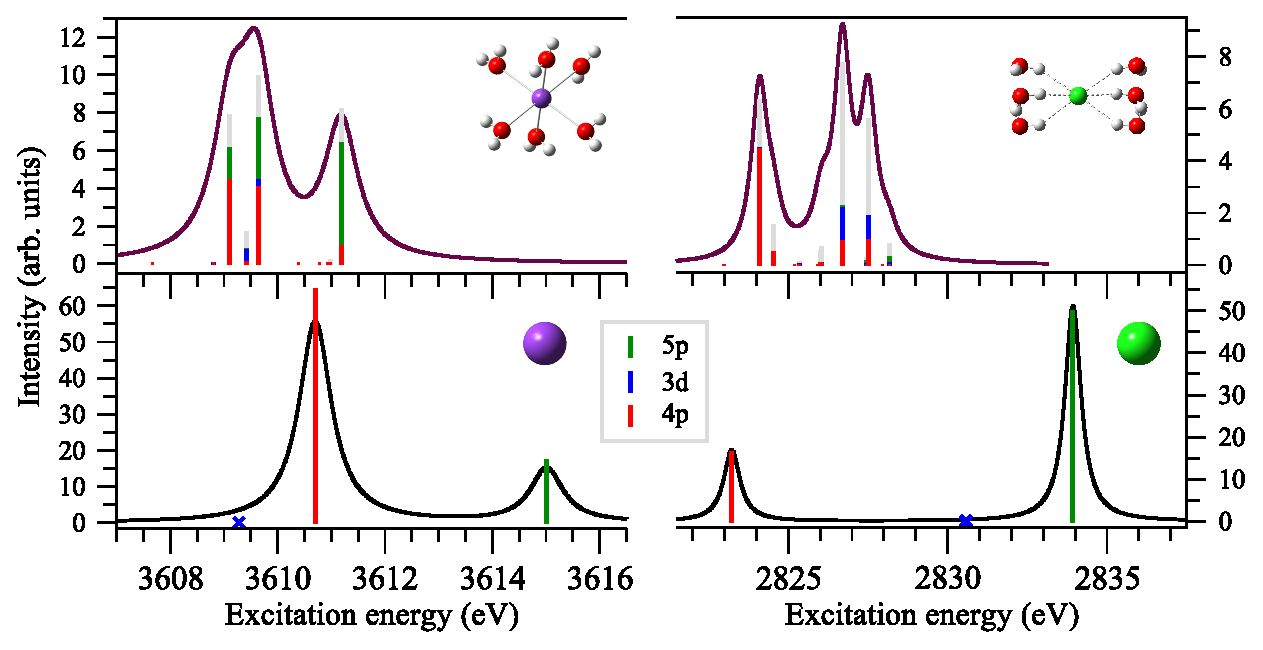
\includegraphics[scale=0.6]{figures/xas_spectra.eps}
\caption{
XAS spectra of the lowest K-shell transitions in the bare K$^{+}$ (lower left panel) and Cl$^{-}$ (lower right panel) ions and their 6-coordinated clusters (upper left panel, \ki(H$_2$O)$_6$, and upper right panel, \cli(H$_2$O)$_6$). The theoretical stick spectra were convolved with a Lorentzian profile of FWHM 0.74\,eV for \ki~and 0.62\,eV for \cli~(dashed line) and a Voigt profile to account for the lifetime broadening and the experimental resolution (full line). The stick spectrum corresponds to the projections $|a_{nl}^{i}|^2$ of the SONOs corresponding to the core excited states of the 6-coordinated clusters on the basis of SONOs corresponding to the 1s$\,\rightarrow\,$3d, 1s$\,\rightarrow\,$4p, and 1s$\,\rightarrow\,$5p states in the bare K$^+$ and \cli~ions (Eq.\ \ref{eq:sono_proj}). The theoretical XAS spectra of both \ki~and \cli~were shifted to higher photon energies such that the excitation energies of the lowest core excited states correspond to the experimentally determined energies -- 3610.7\,eV in the case of \ki, and 2825.2\,eV in the case of \cli. The experimental ionization thresholds are depicted as grey boxes starting at photon energies of 3611.9\,eV (\ki$_{\text{aq}}$) and 2825.4\,eV (\cli$_{\text{aq}}$).}
\label{fg:xas_kcl}
\end{figure}


In order to rationalize the pre-edge region of the experimental XAS spectra and the differences in the AES spectra of \ki$_{\text{aq}}$ and \cli$_{\text{aq}}$, we computed the lowest core excited states of the bare \ki~and \cli~ions and their hexa-coordinated clusters. The theoretical XAS spectra are presented in Fig.\ \ref{fg:xas_kcl}. In the bare ions (lowermost panels on Fig.\ \ref{fg:xas_kcl}), the lowest energy peak corresponds to the dipole allowed 1s$\,\rightarrow\,$4p state. The next dipole allowed state, 1s$\,\rightarrow\,$5p, is located 4.3\,eV and 10.8\,eV higher in the cases of \ki~and \cli, respectively. Together with the two dipole allowed transitions, we show the dipole forbidden 1s$\,\rightarrow\,$3d states of the bare ions as blue crosses at photon energies 3611.17\,eV in the case of \ki~and 2831.68\,eV in the case of \cli, respectively. It is noteworthy that the positions of the 1s$\,\rightarrow\,$4p and 1s$\,\rightarrow\,$3d states are inverted in \ki~and \cli. In the case of Cl$^{-}$ the 1s$\,\rightarrow\,$4p excitation has lower energy and the 1s$\,\rightarrow\,$3d excitation is close to the 1s$\,\rightarrow\,$5p state. On the contrary, in K$^{+}$ the 1s$\,\rightarrow\,$3d excitation has lower energy and lies below the 1s$\,\rightarrow\,$4p state. We note in passing that the intensity of the Cl$^{-}$(1s$\,\rightarrow\,$4p) state is lower than that of the \cli(1s$\,\rightarrow\,$5p) state contrary to what is observed in \ki. This difference can be explained with the lower electron density of the 4p compared to the 5p electron in the region close to the core hole which thus results in the lower oscillator strength of the 1s$\,\rightarrow\,$4p compared to the 1s$\,\rightarrow\,$5p transition in \cli~(see Fig.\ \ref{fg:si_rdens_ions} in SI).


The water molecules in the first solvation shell have several effects on the core excited states. First, upon addition of water molecules, the degeneracy of the 1s$\,\rightarrow\,$4p state is lifted and the intensity of the resulting states in the cluster drops. Moreover, the character of these states changes -- they are no longer of pure atomic character but they rather interact with states of the neighboring water molecules (shown as grey bars) and with other closely lying states of the bare ion, such as the dipole allowed 1s$\,\rightarrow\,$5p and dipole forbidden 1s$\,\rightarrow\,$3d state. Thus, the latter also acquire intensity in the cluster due to mixing with the dipole allowed states in the ligand field of the solvent. A similar effect was observed in the XAS spectra of microsolvated clusters of Na$^{+}$ and Mg$^{2+}$ \citep{miteva16:16671}.


Further we assume that only the lowest peak in the theoretical XAS spectra is populated in the experiment for two reasons. First, due to the lifetime broadening, it spreads over approximately 2\,eV which coincides with the width of the pre-edge structure in the experimental XAS spectra. Second, the splitting between the first core excited state and the ionization threshold in the experiment is 1.2\,eV for \ki~and 0.2\,eV for \cli, and thus it is smaller than the splitting between the first and second peak in the theoretical spectra (1.5\,eV for \ki~and $\sim$3\,eV for \cli, Fig.\ \ref{fg:xas_kcl}). In the 6-coordinated cluster (Fig.\ \ref{fg:xas_kcl} upper left panel), which represents the complete first solvation shell around \ki, the lowest peak in the spectrum contains three states. The lowest and highest lying states are split by approximately 0.5\,eV and they have mixed 4p and 5p character. The low intensity state in between these two states has a predominantly 1s$\,\rightarrow\,$3d character. Since the dispersive feature B appears at lower excitation energies compared to the feature C, we assume that it is produced in the resonant Auger decay of the lowest core excited states of \ki, which are predominantly of 1s$\,\rightarrow\,$4p character. Moreover, we can attribute the feature C to the resonant Auger decay of the low intensity dipole forbidden 1s$\,\rightarrow\,$3d state. Thus, we explain both the energy splitting of $\sim$400\,meV photon energy of the two features, and the fact that island C has lower intensity than feature B.


In the hexa-coordinated cluster of \cli, the solvent molecules have little influence on the position and character of the first peak. Since there are no other ionic states close the 1s$\,\rightarrow\,$4p state in the bare ion, this state preserves its character in the cluster and interacts with states of the nearest water molecules. We attribute the two dispersive features on the 2D map of \cli~ and associated with the $^{1}$S and $^{1}$D terms, to the resonant Auger decay of these core excited states involving mostly the 4p orbitals of chloride. 
% {\color{red}%Since the photon energy step in the experimental spectrum coincides with the splitting between the two dispersive features, we assume that they originate from the decay of the same core excited state.
% We assume that the two dispersive features originate from the decay of the same core excited state, since the photon energy resolution at 2.8\,keV is 0.3\,eV and thus of the same magnitude as the difference between the core excited state and the ionization threshold.
% }


To fully characterize the dispersive features on the experimental 2D maps, we also computed the lowest K$^{2+}$[2p$^{-2}$nl](H$_2$O)$_6$ and Cl$^{0}$[2p$^{-2}$nl](H$_2$O)$_6$ states of the hexa-coordinated clusters corresponding to the lowest final spectator resonant Auger states. They are shown as bars in the upper panels on the experimental resonant Auger spectra on Figs.\ \ref{fg:2dmap_k} and \ref{fg:2dmap_cl}. In both cases, we shifted the lowest 2p$^{-2}$4p states such that they coincide with the maxima of the dispersive features on the high kinetic energy part of the $^1$D main line. Out of all final states we show only the doublets. Since the initial core excited states are populated by photon excitation, only doublet states are efficiently populated in the resonant Auger decay. The 2p$^{-2}$nl states of \ki(H$_2$O)$_6$ and \cli(H$_2$O)$_6$ are substantially different and they reflect the fact that the 3d unoccupied orbitals of \ki~are lower than the 4p orbitals, which is the opposite of what is observed in \cli. 


%As mentioned above, we assume that the island B is produced in the decay of the lowest lying core excited state of the hexa-hydrated \ki~cluster, which is of predominantly 1s$\,\rightarrow\,$4p character. 
As mentioned above, we attribute the island B to the decay of the lowest lying core excited state of the hexa-hydrated \ki~cluster, which is of predominantly 1s$\,\rightarrow\,$4p character. Supposing that this state undergoes mostly pure spectator resonant Auger decay, which is the case of the 1s$\,\rightarrow\,$4p state in the isoelectronic Ar atom \citep{ceolin15:022502}, then the lowest states of 2p$^{-2}$4p character located between 2969 and 2970.5\,eV are populated. As can be seen from the Auger electron spectrum at $h\nu = 3610.7$\,eV (upper panel of Fig.\ \ref{fg:2dmap_k}), the lowest 2p$^{-2}$4p states of \ki(H$_2$O)$_6$ starting at electron energy of 2969\,eV are separated by $\sim$5 and 12-13\,eV from the two groups of 2p$^{-2}$3d states located at higher electron kinetic energies. Thus, the group of 2p$^{-2}$3d states at $\sim$2975\,eV lies closer to the position of island C. Consequently, we attribute this dispersive feature as originating from the resonant Auger decay of the 1s$\,\rightarrow\,$3d state of the 6-coordinated \ki~cluster to the group of 2p$^{-2}$3d states lying around 2975\,eV. The splitting between the 2p$^{-2}$4p and 2p$^{-2}$3d states in our calculation is smaller than the splitting between the islands B and C. This difference may be due to the fact that we do not account for the effect of distant solvent shells in our calculation. Concerning the higher lying group of 2p$^{-2}$3d states at kinetic energies between 2982 and 2983\,eV, we conclude that these states are not populated via the Auger process since no additional experimental features are observed.

% \tsveta{Another argument supporting the attribution of the island C as being of 2p$^{-2}$ 3d character can be found by considering the electron transfer from the water molecules (W) discussed in reference \cite{ceolin17:263003}. As a result of this process, an additional feature A is observed on the low-kinetic energy side of the $^1$D main peak in \ki. This feature has the configuration K$^{2+}$2p$^{-2}$3d W$^{-1}$. ...}
Another argument supporting the attribution of the island C as being of 2p$^{-2}$ 3d character comes from the attribution of the A area as given in reference \cite{ceolin17:263003} and from the energy splitting between A and C. The A area originates from a charge transfer process between water (W) and core excited potassium and has the configuration K$^{2+}$(2p$^{-2}$3d)W$^{-1}$. The ionization potential of water in the liquid phase is about 11 eV which fits well with the observed A-C splitting. Based only on these two simple energetic arguments we can attribute the C island to the a K$^{2+}$ 2p$^{-2}$3d configuration and note that neither 2p$^{-2}$3d nor charge transfer states are present in the Cl$^{-}$ case.


In the Cl$^{0}$[2p$^{-2}$nl](H$_2$O)$_6$ spectrum there are two groups of states split by about 7\,eV (see upper panel of Fig.\ \ref{fg:2dmap_cl}). The lower kinetic energy group corresponds to the 2p$^{-2}$($^1$S)4p states, whereas the higher kinetic energy group corresponds to the 2p$^{-2}$($^1$D)4p states. The splitting between the two groups is in good agreement with the experimental splitting between the dispersive features on the high kinetic energy sides of the $^1$S and $^1$D main peaks. Consequently, we attribute these dispersive features as resulting from the resonant Auger decay of the 1s$\,\rightarrow\,$4p core excited state of \cli$_{\texttt{aq}}$ to the 2p$^{-2}$($^1$S)4p and  2p$^{-2}$($^1$D)4p final states. Similar dispersive features originating from the decay of the Cl (1s$\,\rightarrow\,$4p) state were observed on the 2D map of chloromethane CH$_3$Cl recorded in the vicinity of the Cl K-edge in gas phase \cite{gold16:133001}. In this case, however, additional lower-lying core excited state are observed. They result from excitation to the LUMO of CH$_3$Cl, which is a linear combination of the C 2p and Cl 3p atomic orbitals. Since the 3p shell is fully occupied in \cli, such a core excited state is not observed in our experiment.

% Jan 24 Tsveta: this is already written two paragraphs above.

%{\color{red}we do not say anything about the 3d contribution in blue. Am I correct if I am saying: "The calculated 2p-2 3d states represented by blue vertical lines are not populated during the decay of the first core excited state of solvated chloride involving mostly its 4p orbitals with some water contribution."}

\subsection{Delocalization vs resonant Auger decay}

As mentioned above, the delocalization of core excited electrons in aqueous solutions is ultrafast and as such it competes with the resonant Auger decay. In order to estimate the delocalization rate of the core excited electron at the pre-edges of \ki~and \cli, we used the core-hole clock method as in the reference  \cite{bjorneholm92:1892,karis96:1380}.

In the case of \cli, and contrary to \ki, it was possible to perform the same data treatment as in Ref.\ \cite{ceolin15:022502}, %(\tsveta{do you want to explain this data treatment in 1 sentence. now the reader is forced to check the other paper.}\denis{Tsveta, I think that what is just after the i.e. is enough. If you agree let's see what the others are saying}),
i.e. for each photon energy step, all components of the 2D map shown in Fig.\ \ref{fg:2dmap_cl} were isolated by fitting procedures and their intensity integrated to get a partial electron yield as a function of the photon energy. The result is shown on Fig.\ \ref{fg:si_ct_time} in the SI. The figure shows that there is a large overlap between the resonant and normal Auger contributions, due to the proximity of the resonance to the ionization potential and due to the very short lifetime of the corresponding states. At the specific photon energy corresponding to the lowest core excitation, $h\nu = 2825.2$\,eV (Fig.\ \ref{fg:2dmap_cl}, upper panel) a double-peak structure is observed in the interval of kinetic energies 2380 -- 2385\,eV . The position of the first peak coincides with the main $^1$D line resulting from normal Auger, whereas the second peak at 2383.5\,eV corresponds to the final resonant Auger states 2p$^{-2}$($^1$D)4p. By fitting the peak with two Voigt functions, we determine the ratio of the intensities of these peaks to be $\sim$1. Consequently, the delocalization time is of the same order as the Auger lifetime, i.e.\ $\sim$1\,fs. The fast delocalization in this case is a result of the fact that the energy splitting between the \cli~(1s$\,\rightarrow\,$4p) resonance and the ionization threshold is 0.2\,eV, and thus, smaller than the lifetime broadening of 0.62\,eV.

For potassium the treatment is more complex due to the presence of multiple simultaneous processes -- normal, resonant Auger decay, charge transfer (CT) from solvent. To extract the intensity of each component from the 2D map shown in Fig.\ \ref{fg:2dmap_k}, one needs the spectral fingerprints of each process to be separated. However, as can be seen, this is not the case especially close to threshold in the kinetic energy region 2965 -- 2970\,eV. For instance at 3610.7\,eV photon energy on the high-kinetic-energy side of the 2p$^{-2}$($^1$D) state, there are contributions from the PCI tail and from the dispersive 2p$^{-2}$($^1$D)4p state related to the B island. On the low-kinetic-energy side, the charge transfer process leads to a very large structure that unfortunately cannot be easily simulated by a known profile. However, the 1s core-hole lifetime is shorter for potassium than for chloride (0.9 vs.\ 1\,fs) and moreover, the core excited state appears 1.2\,eV below the ionization threshold whereas it is only 0.2\,eV for chloride. Therefore, one can expect a much less efficient delocalization process compared to \cli$_{\text{aq}}$.

% Jan 24, Tsveta This is Denis' original sentence
%\denis{For potassium the treatment was more complex in reason of multiple overlaps. To extract the intensity of each component of the 2D map shown in figure 2, one needs to isolate them. However this operation was not possible especially close to threshold. On one side of the $^1$D state, there are contributions of the PCI tail and of the dispersive state related to the B island, and on the other side, the charge transfer process leads to a very large structure that unfortunately cannot be easily simulated by a known profile. Below threshold, as for instance at 3610.7eV photon energy, we cannot exclude a superposition of the 2p$^{-2}$($^1$D)4p, 2p$^{-2}$($^1$D) and CT states in the kinetic energy region 2965-2970eV. However, we know that the 1s core-hole lifetime is shorter for potassium than for chloride (0.9 vs. 1fs) and moreover, the core excited state appears 1.2\,eV below the ionization threshold whereas it was only 0.2eV for chloride. Therefore, one can expect a much less efficient delocalization process compared to \cli$_{\text{aq}}$.}
